We have talked about the performance of programs; we mentioned high-performance software. But what do we mean when we say that? Intuitively, we understand that a high-performance program is faster than a program with poor performance, but it doesn't mean that a faster program always has good performance (both programs may have poor performance). 

We have also mentioned efficient programs, but is efficiency the same as high performance? While efficiency is related to performance, it is not exactly the same. Efficiency deals with using resources optimally and not wasting them. An efficient program makes good use of the computational hardware.

On the one hand, an efficient program does not leave available resources idle: if you have a computation that needs to be done and a processor that is  not doing anything, that processor should be executing the code that is waiting to be executed. The idea goes deeper: processors have many computing resources in them, and an efficient program tries to make use of as many of these resources as possible at the same time. On the other hand, an efficient program does not waste resources doing unnecessary work: it does not perform computations that do not need to be done, does not waste memory to store data that is never going to be used, does not send data over the network if it's not needed, and so on. In short, an efficient program does not leave the available hardware idle and does not do any work that doesn't have to be done.

Performance, on the other hand, always relates to some metrics. The most common one is "speed," or how fast the program is. The more rigorous way to define this metric is the throughput, which is the amount of computations the program does in a given time. The inverse metric that is often used for the same purpose is the turnaround time or how much time is needed to compute a particular result. However, this is not the only possible definition of performance.

\subsubsubsection{1.3.1\hspace{0.2cm}Performance as throughput}

Let's consider four programs that use different implementations to compute the same end result. Here are the run times of all four programs (units are relative; the actual numbers don't matter as we're interested in relative performance):

\hspace*{\fill} \\ %插入空行
\begin{center}
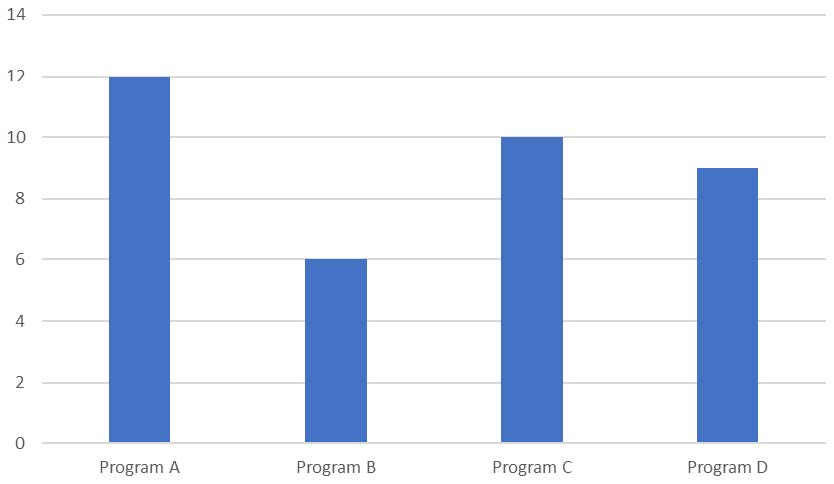
\includegraphics[width=0.9\textwidth]{content/1/chapter1/images/5.jpg}\\
Figure 1.5 – Run times of four different implementations of the same algorithm (relative units)
\end{center}

It seems obvious that Program B has the highest performance: it finished before the other three programs, in half the time it took the slowest program to compute the same result. In many situations, this would be all the data we need to choose the best implementation.

But the context of the problem matters, and we neglected to mention that the program is running on a battery-powered device, such as a cell phone, and the power consumption matters as well.

\subsubsubsection{1.3.2\hspace{0.2cm}Performance as power consumption}

Here is the power consumed by all four programs during the course of the computation:

\hspace*{\fill} \\ %插入空行
\begin{center}
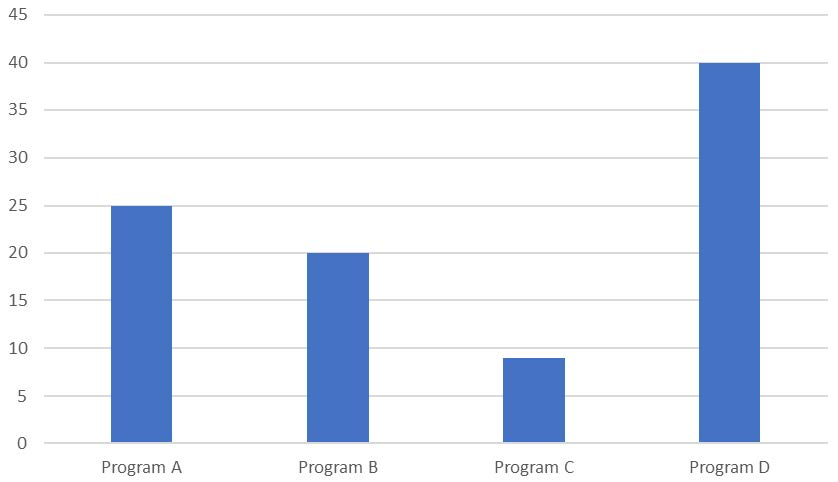
\includegraphics[width=0.9\textwidth]{content/1/chapter1/images/6.jpg}\\
Figure 1.6 – Power consumption of four different implementations of the same algorithm (relative units)
\end{center}

Despite taking longer to get the result, Program C used less power overall. So, which program has the best performance? 

Again, this is a trick question without knowing the full context. The program not only runs on a mobile device but performs a real-time computation: it is used in audio processing. This should put a premium on getting the results back faster in real time, right? Not exactly.

\subsubsubsection{1.3.3\hspace{0.2cm}Performance for real-time applications}

A real-time program must keep up with the events it is processing at all times. An audio processor must keep up with speech, in particular. If the program can process audio ten times faster than a person can speak, it does us no good, and we may as well turn our attention to power consumption.

On the other hand, if the program occasionally falls behind, some sounds or even words will be dropped. This suggests that the real time, or speed, matters up to a point, but it must be delivered in a predictable manner.

There is, of course, a performance metric for that as well: the latency tail. The latency is the delay, in our case, between the time the data is ready (voice recorded) and the time when the processing is completed. The throughput metric we saw earlier reflects the average time to process the sound: if we speak for one hour into the phone, how long will it take for the audio processor to do all the computations it needs to do? But what really matters in this context is that each little computation for every sound is done on time. 

At a low level, the computation speed fluctuates: sometimes, the computation finishes faster, and sometimes it takes longer. As long as the average speed is acceptable, what matters are the rare long delays.

The latency tail metric is computed as a particular percentile of the delay, for example, at the 95th percentile: if t is the 95th percentile latency, then 95\% of all computations take less time than t. The metric itself is the ratio of the 95th percentile time t to the average compute time t0 (it is often expressed as a percentage as well, so a 30\% latency at the 95th percentile means that t is 30\% greater than t0):

\hspace*{\fill} \\ %插入空行
\begin{center}
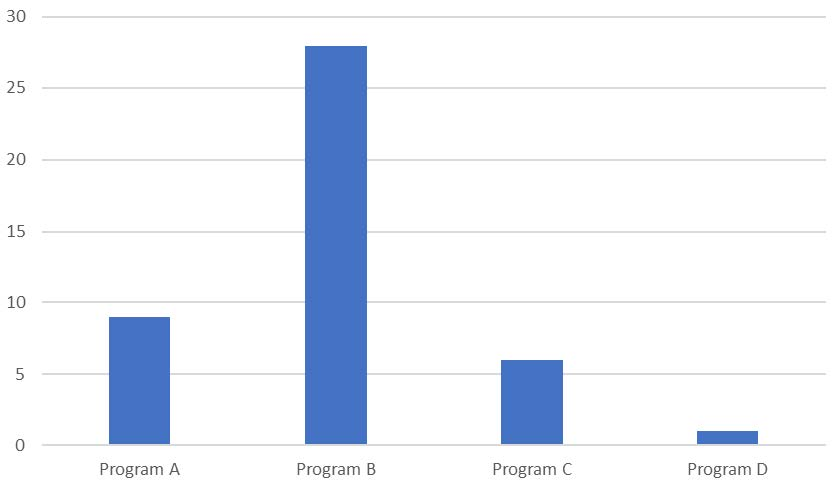
\includegraphics[width=0.9\textwidth]{content/1/chapter1/images/7.jpg}\\
Figure 1.7 – 95\% latency of four different implementations of the same algorithm (percents)
\end{center}

We now see that Program B, which computes the results faster than any other implementation, on average, also delivers the most unpredictable run time results, while Program D, which never stood out before, computes like clockwork and takes practically the same time to do a given computation, every time. As we have already observed, program D also has the worst power consumption. This is, unfortunately, not uncommon because the techniques that make the program more power-efficient, on average, are probabilistic in nature: they speed up the computations most of the time, but not every time.

So, which program is the best? The answer, of course, depends on the application and even then may be non-obvious.

\subsubsubsection{1.3.4\hspace{0.2cm}Performance as dependent on context}

If this was simulation software that runs in a large data center and takes days to compute, the throughput would be the king. On a battery-powered device, power consumption is usually the most important. In a more complex environment, such as our real-time audio processor, it is the combination of multiple factors. The average run time matters, of course, but only until it becomes "fast enough." If the speaker cannot notice the delays, then making it even faster has no reward. Latency tail matters: users hate it when a word is dropped from the conversation every now and then. Once the latency is good enough that the call quality is limited by other factors, improving it further gives very little benefit; we would be better off conserving power at this point.

We now understand that, unlike efficiency, performance is always defined with respect to specific metrics, that these metrics depend on the application and the problem we're solving, and that for some metrics, there is such a thing as "good enough" when other metrics come to the foreground. The efficiency, which reflects the utilization of the computational resources, is one of the ways to achieve good performance, the most common way, perhaps, but not the only one.












